\section{Discussion}
 
\subsection{Synthesis of Key Findings}
 
Collectively, the three research questions reveal a field in active and accelerating development, characterised by increasing methodological sophistication and a clear orientation toward preemptive risk management over reactive recovery. The literature converges strongly on early warning and forecasting as the primary mode of AI-enabled risk mitigation~\cite{deivaganesh2022future}~\cite{li2025endtoend}~\cite{farzhana2025hybrid}, reflecting a theoretical consensus that the most effective supply chain risk management intervenes before disruptions propagate through the network.
 
The cross-reference matrix (Fig.~\ref{fig:heatmap}) reveals structural patterns in the relationship between AI techniques and risk types. Traditional machine learning dominates across the broadest risk portfolio, reflecting its versatility for structured operational data. Deep Learning and hybrid architectures concentrate on disruption, logistics, and demand risks, which are characterised by temporal complexity and high data volume. Generative AI and Knowledge Graphs are emerging in fraud and integrity risk contexts, where the capacity to reason over unstructured information and relational knowledge is particularly valuable. XAI techniques are distributed across supplier, pandemic, and geopolitical risks, confirming that high-stakes, low-frequency risk decisions create the strongest demand for interpretable AI outputs.
 
The dominance of logistics and transport risk and disruption risk in the cross-reference matrix, relative to the near-absence of cybersecurity, geopolitical, and fraud risks, reveals a field that is strongly responsive to operationally visible and historically recent disruptions, while exhibiting limited engagement with risks that are either diffuse, novel, or difficult to quantify from structured data alone.
 
% ----------------------------------------
 
\subsection{Emerging Trends}
 
\textit{Transition from single-model to multi-agent architectures.} The most architecturally ambitious contributions of 2025 deploy systems in which multiple specialised AI components perform distinct functions within a unified pipeline. Rajesh et al.~\cite{rajesh2025smartops} integrate an LLM, Random Forest, K-Means, an LSTM autoencoder, and Reinforcement Learning within a single multi-agent framework. Lin et al.~\cite{lin2025generative} combine Generative AI, Markov modelling, and Mixed Integer Programming. This represents a qualitative departure from the single-model approaches predominant in 2022 and 2023 articles and suggests a trajectory toward integrated supply chain risk intelligence platforms.
 
\textit{Entry of Generative AI and LLMs into supply chain risk management.} Two 2025 articles deploy Large Language Models as active components of risk management architectures~\cite{lin2025generative}~\cite{rajesh2025smartops}, a development with no precedent in earlier articles of the corpus. The capability of LLMs to extract structured risk signals from unstructured text (news, regulatory updates, supplier communications) addresses a longstanding limitation of traditional ML approaches, which require structured input data. This trend is likely to intensify as domain-specific fine-tuning and retrieval-augmented generation techniques lower the cost of deploying LLMs in operational contexts.
 
\textit{Growth of explainability as a design requirement.} The increasing prevalence of SHAP and LIME-based interpretability frameworks (evidenced in articles by Adom et al.~\cite{adom2025design}, Kumar and Kumar~\cite{kumar2023enhancing}, Li et al.~\cite{li2025endtoend}, and the systematic review by Nimmy et al.~\cite{nimmy2022explainability}) signals that explainability has transitioned from an optional enhancement to a first-class design requirement. This reflects the practical reality that supply chain risk decisions carry significant financial and operational consequences, requiring not only accurate predictions but transparent justifications that managers can act upon and audit.
 
\textit{Post-COVID-19 acceleration and diversification of risk categories studied.} The temporal distribution confirms the COVID-19 pandemic as a research accelerant, generating both the empirical urgency and the data availability needed to develop and validate AI-based risk management systems. Post-2022 articles begin to diversify beyond pandemic risk into geopolitical risk~\cite{aldehayyat2025applying}, fraud and integrity risk~\cite{lin2025generative}, and ESG-related risk~\cite{rajesh2025smartops}, suggesting that the field is broadening its risk aperture beyond the immediate disruption context.
 
% ----------------------------------------
 
\subsection{Identified Gaps}
 
The research gaps identified across the corpus are summarised in Fig.~\ref{fig:gaps} and discussed below.
 
\begin{figure}[H]
  \centering
  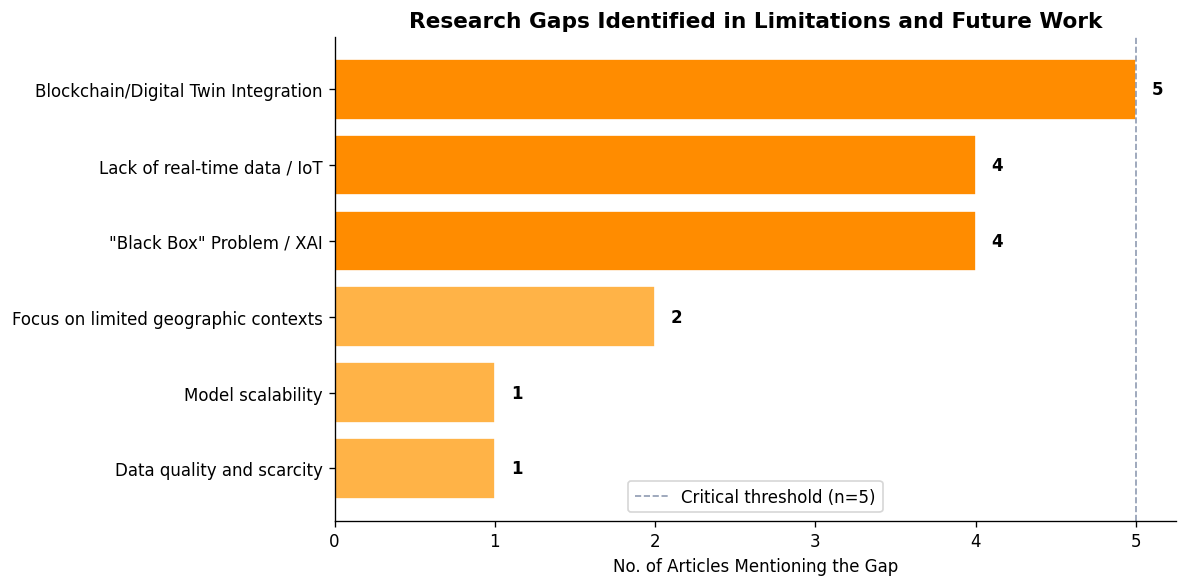
\includegraphics[width=\linewidth]{figures/fig_gaps.png}
  \caption{Research gaps identified across the included articles, ranked by frequency of mention.}
  \label{fig:gaps}
\end{figure}
 
\textit{Blockchain and Digital Twin integration} is the most frequently identified gap, mentioned in five articles. The literature consistently notes that AI-based risk management systems would benefit substantially from integration with blockchain for immutable audit trails and Digital Twin environments for real-time simulation of disruption scenarios~\cite{fernando2024covid}~\cite{nguyen2024federated}~\cite{yang2024building}. The absence of empirical studies implementing such integrations at operational scale represents the most prominent frontier for future research.
 
\textit{Lack of real-time data and IoT integration} is cited in four articles as a barrier to the operationalisation of AI risk management frameworks. Many proposed models are validated on historical batch datasets rather than live operational streams, limiting their applicability for real-time early warning~\cite{deivaganesh2022supply}~\cite{yang2025design}. Future research should prioritise architectures that ingest IoT sensor data, RFID streams, and other real-time supply chain telemetry.
 
\textit{The black box problem and the need for XAI} is identified in four articles as a critical barrier to managerial adoption~\cite{nimmy2022explainability}~\cite{kumar2023enhancing}~\cite{li2025endtoend}~\cite{adom2025design}. Despite the growing prevalence of SHAP-based interpretability in recent contributions, the majority of proposed AI systems still lack sufficient transparency for deployment in regulated or safety-critical supply chain environments. Developing explainability frameworks specifically tailored to supply chain risk contexts remains an open research challenge.
 
\textit{Focus on limited geographic contexts} is noted in two articles~\cite{yang2025design}~\cite{nguyen2024federated}. The concentration of empirical studies in Asian manufacturing and logistics contexts limits the generalisability of findings to supply chains operating under different regulatory frameworks, infrastructure conditions, and risk exposure profiles. Studies conducted in European, North American, and developing-economy contexts are needed to establish the cross-contextual validity of AI-based risk management frameworks.
 
\textit{Model scalability} and \textit{data quality and scarcity} are each identified in one article as constraints on the practical deployment of AI systems~\cite{li2025endtoend}~\cite{deivaganesh2022future}. Supply chain disruption events are rare and high-impact, creating class-imbalance problems that undermine the reliability of models trained on historical data. Techniques for few-shot learning, synthetic data generation, and transfer learning across supply chain domains represent promising avenues for addressing these constraints.
 
% ----------------------------------------
 
\subsection{Limitations of This Review}
 
This review is subject to several limitations that should be considered when interpreting its findings. First, the literature search was restricted to two databases (IEEE Xplore and Web of Science), which, while chosen for their complementary technical and multidisciplinary coverage, may have excluded relevant contributions indexed in Scopus, the ACM Digital Library, or domain-specific repositories. Second, the time restriction to 2019 and 2025 excludes foundational work published prior to 2019 that may underpin more recent methodological contributions. Third, the language restriction to English and Portuguese may introduce a systematic bias against research communities publishing in Mandarin, Arabic, or other languages, which is particularly relevant given the geographic concentration of the corpus in Asia. Finally, the classification of AI techniques and risk types relied in some instances 
on abstract-level metadata rather than deep full-text algorithmic audits, which may  have introduced minor categorisation imprecision. 
 